\documentclass{article}
\usepackage{amsmath}
\usepackage{cite}
\usepackage{amssymb}
\usepackage{amsfonts}
\usepackage{graphicx}
\usepackage{textcomp}
\usepackage{xcolor}
\usepackage{subcaption}
\usepackage{float}

\begin{document}

\title{Classificador bayesiano no dataset Parkinson.}

\author{Arthur Felipe Reis Souza \\
Electrical Engineering Department, \\
Federal University of Minas Gerais, \\
Belo Horizonte, Brazil \\
arthurfreisouza@gmail.com \\
\and
Antônio de Pádua Braga and Frederico Gualberto Ferreira Coelho \\
Electrical Engineering Department, \\
Federal University of Minas Gerais, \\
Belo Horizonte, Brazil \\
apbraga@cpdee.ufmg.br, fredgfc@ufmg.br
}

\maketitle

\begin{abstract}
   % Abstract content here.
\end{abstract}

\section{Introdução}

Este relatório tem por objetivo mostrar o processo de classificação utilizando a regra de Bayes como base, onde o conjunto são características que descrevem a doença de Parkinson.

\section{Dados}

Os dados são obtidos no site https://archive.ics.uci.edu/dataset/174/parkinsons, e contém 197 instâncias de 23 variáveis. O objetivo do estudo é, com base nas características, concluir se um paciente tem ou não a doença de Parkinson. Para isso, o classificador Multivariado de Bayes foi utilizado.

 \section{Aplicação do algoritmo}

 O classificador bayesiano leva em consideração a independência entre os atributos, bem como a probabilidade a priori de ocorrência da classe ao realizar a classificação. Ele se baseia no teorema de Bayes, que é descrito pela seguinte equação:
 
 \[
P(C|X) = \frac{P(X|C) \cdot P(C)}{P(X)}
\]

Apesar de considerar a independência entre as características, o mesmo pode ser extendido para casos onde há uma certa correlação entre os atributos. Nesses casos, o classificador irá considerar a matriz de covariâncias na estimativa da função densidade.

\begin{figure}[h]
    \centering
    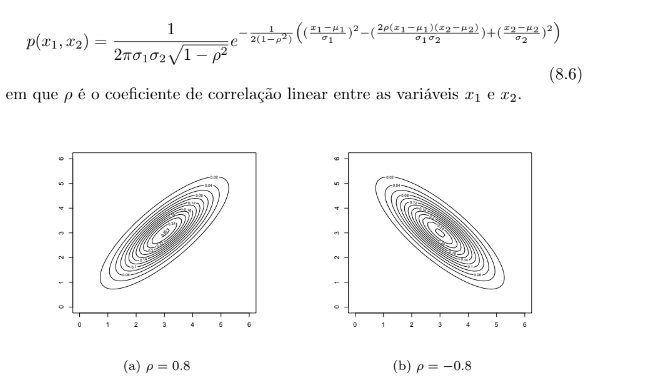
\includegraphics[width=0.75\linewidth]{caso_geral_bayes.png}
    \caption{Equação geral da estimativa do classificador de bayes Multivariado.}
    \label{fig:kernel_types}
 \end{figure}

\section{Resultados}

Após aplicar o classificador bayesiano na base de dados Parkinson, utilizando o K-Fold Cross Validation, com K = 10, obtemos que a acurácia de 70\%. Ao desconsiderar o K-Fold e separar os dados em treino e teste, a seguinte matriz de confusão foi obtida : 

\begin{figure}[h]
    \centering
    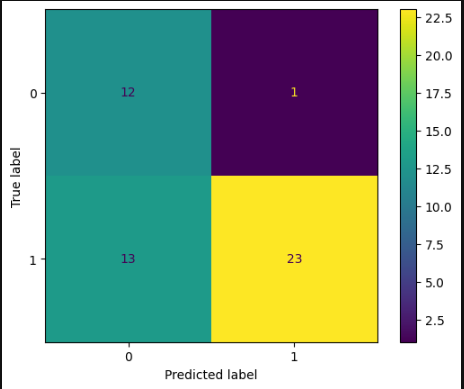
\includegraphics[width=0.75\linewidth]{conf_mat.png}
    \caption{Matriz de confusão classificador de bayes na base de dados Parkinson.}
    \label{fig:kernel_types}
 \end{figure}

O classificador não obteve um bom desempenho. Ele está classificando pessoas que tem parkinson como pessoas que não tem.

\section{Conclusão}

Com este relatório, foi possível aplicar o classificador Bayesiano na base de dados de Parkinson. Os resultados obtidos mostram que o classificador teve um bom desempenho ao identificar pessoas com a doença. No entanto, ele classificou erroneamente 13 pessoas como não tendo a doença, quando na verdade elas a possuem. Problemas como esses nos levam a refletir sobre a importância de uma análise mais profunda das métricas a serem consideradas. Afinal, seria menos prejudicial classificar 13 pessoas como tendo Parkinson, quando elas não têm, do que cometer o erro oposto e classificar pessoas que realmente possuem a doença como se não tivessem.

\end{document}
